\documentclass[]{article}
\renewcommand{\baselinestretch}{1.25}

\usepackage[margin=1in]{geometry}
\usepackage{physics}
\usepackage{amsmath, amsfonts, amssymb, amsthm}
\usepackage{amssymb}
\usepackage{graphicx}
\usepackage{hyperref}
\usepackage{empheq}
\usepackage{pdfpages}
\usepackage{xcolor}
\usepackage{ulem}

% MATLAB Formatting Code
\usepackage[numbered,framed]{matlab-prettifier}
\lstset{style=Matlab-editor,columns=fullflexible}
\renewcommand{\lstlistingname}{Script}
\newcommand{\scriptname}{\lstlistingname}

% TikZ Things
\usepackage{tikz}
\usetikzlibrary{positioning,shapes}


% Formatting Preferences
\numberwithin{equation}{section}
\usepackage{parskip}
\renewcommand{\figurename}{Fig.}
\allowdisplaybreaks

% Section Heading Settings
\usepackage{enumitem}
\renewcommand{\theenumi}{\alph{enumi}}
\renewcommand*{\thesection}{Problem \arabic{section}}
\renewcommand*{\thesubsection}{\alph{subsection})}
\renewcommand*{\thesubsubsection}{\quad \quad \roman{subsubsection})}

% Math Proof things
\newcommand{\Rel}{\mathcal{R}}
\newcommand{\R}{\mathbb{R}}
\newcommand{\C}{\mathbb{C}}
\newcommand{\N}{\mathbb{N}}
\newcommand{\Z}{\mathbb{Z}}
\newcommand{\Q}{\mathbb{Q}}

\newcommand{\st}{\ : \ }

% Theorem Definition
\newtheorem{definition}{Definition}
\newtheorem{assumption}{Assumption}
\newtheorem{theorem}{Theorem}
\newtheorem{lemma}{Lemma}
\newtheorem{proposition}{Proposition}
\newtheorem{example}{Example}


% Multiagent Robotic Systems Commands
\newcommand{\diam}{\textnormal{diam}}
\newcommand{\radius}{\textnormal{radius}}




%opening
\title{MECH 6V29: Multiagent Robotic Systems- HW 3}
\author{Jonas Wagner}
\date{2022, March 22\textsuperscript{nd}}

\begin{document}	

\maketitle

\tableofcontents

%----------------------------------------------------------------------------
\newpage
\section*{Preliminary Notes}

\subsection{Definitions}
\begin{definition} \label{def:graph_def}
	\underline{\emph{Graph}} $G(V,E)$ is constructed with \underline{\emph{vertex set}} \[
		V = \qty{v_1,v_2,\dots,v_n}
	\] of $n$ discrete vertices and \emph{\underline{edge set}} \[
		E = \qty{e_1, \dots, e_m} \subseteq V \cross V
	\] consisting of $m$ edges $e_{k=(i,j)} = (v_i,v_j) \forall_{k=1,\dots,m}$ connecting vertices $v_i$ and $v_j$.
\end{definition}

\begin{definition} \label{def:graph_properties}
	Let graph $G(V,E)$ with $V = \qty{v_1,\dots,v_n}$ and $E \subseteq V \cross V$.
	\begin{enumerate}
		\item $G(V,E)$ is considered \underline{\emph{undirected}} if\[
			(v_i,v_j) \in E \iff (v_j,v_i) \in E
		\] otherwise, $G(V,E)$ is considered \emph{directed}.
		\item An undirected graph $G(V,E)$ is considered \underline{\emph{connected}} if there exists a path between any two vertices.
		\item A directed graph $G(V,E)$ is considered \underline{\emph{strongly connected}} if there exists a directed path between any two vertices.
		\item A directed graph $G(V,E)$ is considered \underline{\emph{weakly connected}} if the corresponding undirected graph is connected.
	\end{enumerate}
\end{definition}

\begin{definition} \label{def:graph_matrices}
	Let graph $G(V,E)$ with $V = \qty{v_1,\dots,v_n}$ and $E \subseteq V \cross V$.
	\begin{enumerate}
		\item The \underline{\emph{degree matrix}} $\Delta \in \R^{n\cross n}$ is a diagonal matrix defined as \[
			\Delta := \mqty[\dmat{\deg(v_1), \deg(v_2), \ddots, \deg(v_n)}]
		\]
		\item The \emph{\underline{adjacency matrix}} $A \in \R^{n\cross n}$ is a symmetric matrix $(A = A^T)$ defined s.t. \[
			A = [a_{ij}] \st a_{ij} \begin{cases}
				1 &(v_i,v_j) \in V\\
				0 &(v_i,v_j) \notin V
			\end{cases}
		\]
		\item The \emph{\underline{incidence matrix}} $D \in \R^{n \cross m}$ is defined as\[
			D = [d_{ij}] \st d_{ij} \begin{cases}
				1 	&(v_i,-) \in e_{j}\\
				-1	&(-,v_i) \in e_{j}\\
				0	&\text{otherwise}
			\end{cases}
		\]
		\item The \emph{\underline{Laplacian matrix}} $L \in \R^{n \cross n}$ is a symmetric $(L = L^T)$ and strictly semi-positive definite $(L \succeq 0)$ is defined as\[
			L := \Delta - A = D D^T
		\]and\[
			L = \mqty[
				\deg(v_1)	&-a_{12}	&-a_{13}	&\cdots	&-a_{1n}\\
				-a_{21}		&\deg(v_2)	&-a_{23}	&\cdots	&-a_{2n}\\
				\vdots		&\vdots		&\vdots		&\ddots	&\vdots\\
				-a_{n1}		&-a_{n2}	&-a_{n3}	&\cdots	&\deg(v_n)
			]
		\]
		\item For a weighted graph $G(V,E,W)$, the diagonal weighted matrix $W\in \R^{m\cross m}$ is defined as\[
			W = [w_{ij}] \forall_{ij \in E}
		\]
		were $w_{ij}$ are the corresponding weights for $e_{ij} = (v_i,v_j)$.
	\end{enumerate}
\end{definition}

\begin{definition} \label{def:consensus_dynamics}
	Let undirected and unweighted graph $G(V,E)$ with $V = \qty{v_1,\dots,v_n}$ and $E \subseteq V \cross V$.
	The \emph{\underline{consensus dynamics}} of network $G(V,E)$ is defined by\[
		\forall_{i=1,\dots,n} \ \dot{x}_i = \sum_{j\in \mathcal{N}_i} (x_j - x_i)
		\iff \dot{x} = -L x
	\] For the case with weighted graph $G(V,E,W)$ with diagonal weight matrix $W = [w_{ij}]$, 
	\emph{\underline{weighted consensus dynamics}} are given as\[
		\dot{x}_i = \sum_{j\in\mathcal{N}_i} w_{ij} (x_j - x_i) 
		\implies \dot{x} = - L_{w} x
	\]where weighted Laplacian matrix $L_{w}$ is defined as\[
		L_{w} = D W D^T
	\]
\end{definition}





% \begin{definition}\label{def:Delta-disk_graph}
% 	Let $V = \qty{v_1,v_2,\dots,v_n}$ be vertices.
% 	\emph{\underline{$\Delta$-Disk Graphs}} are constructed for a particular $\Delta$ such that \[
% 		(v_i,v_j) \in E \iff \norm{v_i,v_j} \leq \Delta
% 	\]
% \end{definition}


% \begin{definition}\label{def:path_diam_radius_etc}
% 	Let $G(V,E)$ be a undirected graph with $V = \qty{v_1,v_2,\dots,v_n}$ 
% 	and $E = \qty{e_1, \dots, e_m} \subseteq V \cross V$ 
% 	with $e_k = e_{ij} = (v_i, v_j)$.
% 	\begin{enumerate}
% 		\item A \emph{\underline{path}} between two vertices $v_i$ and $v_j$ is a sequence of edges $[e_{i, *}, \dots, e_{*, j}]$ that joins a sequence of vertices $[v_i, \dots, v_j]$.
% 		\item A \emph{\underline{path length}} is the number of edges in the path. 
% 		\item The \emph{\underline{shortest path length}} $l_{i,j}$ is the minimum length of all paths between vertices $v_i$ and $v_j$. 
% 		This quantity is also known as the \emph{\underline{distance}} between $v_i$ and $v_j$, $\text{dist}\qty(v_i,v_j)$.
% 		\item The \emph{\underline{diameter}} of graph $G(V,E)$ is the maximum distance between any two vertices in the graph. 
% 		(i.e.)\[
% 			\diam(G(V,E)) := \max_{v_i,v_j \in V} l_{i,j}
% 		\]
% 		\item The \emph{\underline{eccentricity}} of vertex $v_i$, $l_{i}^{*}$, is the largest distance from $v_i$ to any other vertex in the graph. 
% 		(i.e)\[
% 			l_{i}^{*} := \max_{v_j \in V} l_{i,j}
% 		\]
% 		\item The \emph{\underline{radius}} of graph $G(V,E)$ is the minimum eccentricity of the vertices of the graph.
% 		(i.e)\[
% 			\radius(G(V,E)) := \min_{v_i \in V} l_{i}^{*} = \min_{v_i \in V} \max_{v_j \in V} l_{i,j}
% 		\]
% 	\end{enumerate}
% \end{definition}



% \begin{definition}\label{def:leader_follower_dynamics}
%     Let undirected and unweighted graph $G(V,E)$ with $V = \qty{v_1,\dots,v_n}$ and $E \subseteq V \cross V$.
%     Vertices in $V$ are classified as either \emph{leaders} ($v_i \in V_l$) or \emph{followers} ($v_i \in V_f)$. 
% 	The \emph{\underline{leader-follower}} dynamics of the states within network $G(V,E)$ are defined by\[\begin{cases}
%         \dot{x}_i = - \sum_{j \neq N_i} (x_i - x_j) &\forall_{i \st v_i \in V_{f}}\\
%         \dot{x}_i =  0 &\forall_{i \st v_i \in V_{l}}
%     \end{cases}
% 	\] or equivalently when $V_{l} = \{v_n\}$ (single leader node) \[
%         \dot{x} = \mqty[
%             -L_f & - l\\
%             0 & 0
%         ]
%     \]
% \end{definition}


% --------------- Directed consensus....
% \begin{definition} 
%     Let directed network (di-graph) $G(V,E)$ with $V = \qty{v_1,\dots,v_n}$ and $E \subseteq V \cross V$.
%     \begin{enumerate}
%         \item A directed path ($P : v_i \to v_j$) is a sequence of directed edges constructing a path from $v_i$ to $v_j$.
%         \item 
%     \end{enumerate}
% \end{definition}

% \begin{definition}
%     \textbf{Connectivity of Directed Graphs:} 
%     Let directed network (di-graph) $G(V,E)$ with $V = \qty{v_1,\dots,v_n}$ and $E \subseteq V \cross V$.
%     \begin{enumerate}
%         \item Di-graph $G(V,E)$ is \emph{\underline{strongly connected}} there exists a directed path from any node to every other node.
%         \item Di-graph $G(V,E)$ is \emph{\underline{weakly connected}} the corresponding undirected graph is connected.
%         \item Di-graph $G(V,E)$ is contains a \underline{\emph{rooted out-branching}} if \begin{enumerate}
%             \item $G(V,E)$ does not contain a directed cycle
%             \item $\exists_{v_r \in V}$ such that $\forall_{v_i \neq v_r \in V}$ there is a directed path from $v_r$ to $v_i$.
%         \end{enumerate}
%         \item  Di-graph $G(V,E)$ is considered \underline{\emph{balanced}} if $\deg^{in}(v_k) = \deg^{out}(v_k) \forall_{v_k \in V}$.
%     \end{enumerate}
% \end{definition}

% \begin{theorem}
%     \textbf{Consensus Requirements:}
%     Let directed network (di-graph) $G(V,E)$ with $V = \qty{v_1,\dots,v_n}$ and $E \subseteq V \cross V$
%     \begin{enumerate}
%         \item 
%         \item Di-graph $G(V,E)$ drives to $x$ to $\frac{1}{N} \vb{1} \vb{1}' x(0)$ iff $L$ is balanced and contains a rooted out-branching.
%     \end{enumerate}
% \end{theorem}




% Include Switched Systems & Lyapnov stability....












% Problem 1 -------------------------------------------------
\newpage
\section{}
State a summary of \emph{\textbf{Notes 11, 12 and 13}}, preferably by creating a concept map diagram (flow diagram). 
The whole purpose is to make sure that we are clear about the bigger picture, 
and reiterate why are we doing and discussing the specific topics in the class. 
Do not merely write the topics, instead create connections between topics to clarify the flow of information.

\textbf{Note:} 
Since we have only covered Notes 11 and 12, this chart only includes those topics.

\subsection{Big Picture Chart}
\begin{figure}[h]
	\centering
    \resizebox*{\textwidth}{!}{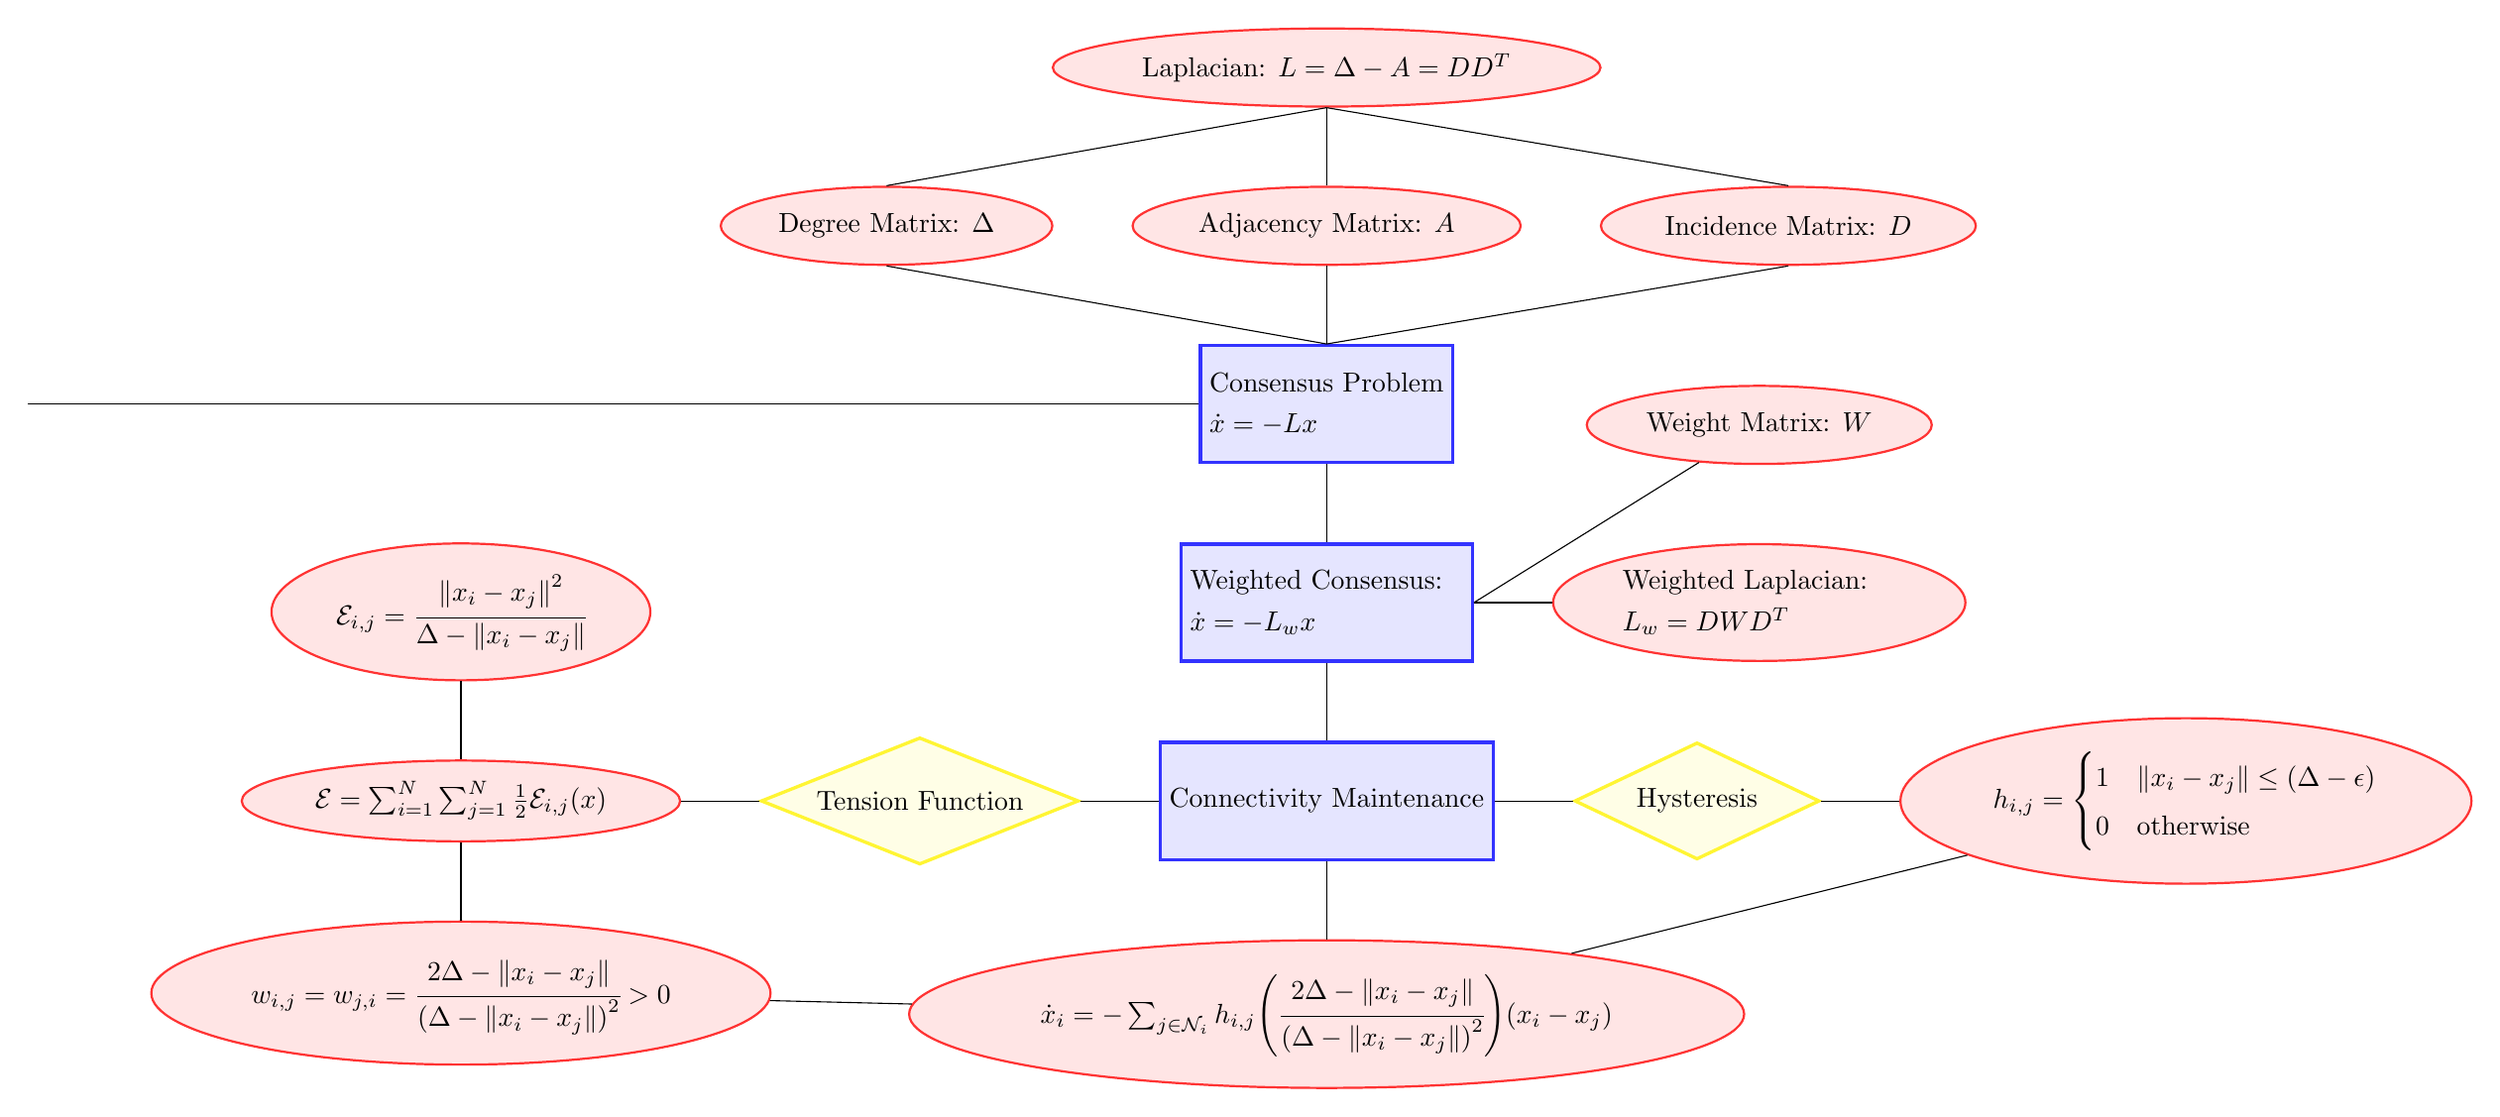
\begin{tikzpicture}[
		empty/.style={coordinate, draw=white!0, fill=white!0, thin, minimum size = 0.1mm},
		block/.style={rectangle, draw=blue!80, fill=blue!10, very thick, minimum size = 15mm},
        subblock/.style={diamond, draw=yellow!80, fill=yellow!10, very thick, minimum size = 15mm, aspect=2.5},
		extra/.style={ellipse, draw=red!80, fill=red!10, thick, minimum size = 10mm},
		auto,
		% roundnode/.style={circle, draw=green!60, fill=green!5, very thick, minimum size=7mm},
		% squarednode/.style={rectangle, draw=red!60, fill=red!5, very thick, minimum size=5mm},
		]
		%Main Nodes
		\node[empty]	(center)								{};
		
        % %Consensus
        \node[block, text width = 30mm]	(consensus)	[above=2cm of center]	{Consensus Problem $\dot{x}=-L x$};
        \node[extra]	(con_2)		[above=of consensus]	{Adjacency Matrix: $A$};
        \node[extra]	(con_1)		[left=of con_2]			{Degree Matrix: $\Delta$};
        \node[extra]	(con_3)		[right=of con_2]		{Incidence Matrix: $D$};
        \node[extra]	(con_4)		[above=of con_2]		{Laplacian: $L = \Delta - A = DD^T$};
        \draw[-]	(consensus.north) 	--	(con_1.south);
        \draw[-]	(consensus.north) 	--	(con_2.south);
        \draw[-]	(consensus.north) 	--	(con_3.south);
        \draw[-]	(con_1.north)		--	(con_4.south);
        \draw[-]	(con_2.north)		--	(con_4.south);
        \draw[-]	(con_3.north)		--	(con_4.south);

        % %Directed Consensus
        % \node[subblock]	(di_con)	[right=of consensus]	{Directed Consensus};
        % \draw[-]    (consensus.east) -- (di_con.west);
        % \node[extra]    (di_con_1)  [right=of di_con]    {Strongly vs Weakly Connected};
        % \draw[-]    (di_con.east) -- (di_con_1.west);
        % \node[extra]    (di_con_2)  [below=of di_con_1]    {Rooted Out-branching};
        % \draw[-]    (di_con.east) -- (di_con_2.west);

        %Weighted Consensus
        \node[block, text width = 35mm]	(w_con)	[below=of consensus]	{Weighted Consensus: $\dot{x} = -L_{w} x$};
        \draw[-]    (consensus.south) -- (w_con);
        \node[extra, text width = 35mm]    (w_con_2)  [right=of w_con]    {Weighted Laplacian: $L_{w} = D W D^{T}$};
        \draw[-]    (w_con.east) -- (w_con_2);
        \node[extra]    (w_con_1)  [above=of w_con_2]    {Weight Matrix: $W$};
        \draw[-]    (w_con.east) -- (w_con_1);
        % \node[extra]    (w_con_3)  [below=of w_con_2]    {Static \& Dynamic Weights};
        % \draw[-]    (w_con.east) -- (w_con_3.west);

        % %Time-Varying Consensus
        % \node[subblock]	(tv_con)	[left=of consensus]	{Time Varying Consensus};
        % \draw[-]    (consensus.west) -- (tv_con.east);
        % \node[extra]    (tv_con_1) [left=of tv_con] {Switched Networks};
        % \draw[-]    (tv_con.west) -- (tv_con_1.east);
        % \node[extra, text width = 40mm]    (tv_con_2) [below=of tv_con_1] {Universal vs Existential Stability};
        % \draw[-]    (tv_con.west) -- (tv_con_2.east);

        % %Lyapnov Stability
        % \node[block]	(lyap)		[left=3cm of center] 	{Lyapnov Stability};
        % \draw[-]    (lyap.west) -- (tv_con_2.east);
        % \draw[-]    (lyap.north) -- (consensus.south);

        % %Leader-Follower System
        % \node[block]	(lead_follow)		[right=3cm of center] 	{Leader-Follower Network};
        % \draw[-] (consensus.south) -- (lead_follow.north);

        %Connectivity Maintenance
        \node[block]	(cnct_maint)    [below=of w_con] 	{Connectivity Maintenance};
        \draw[-] (w_con.south) -- (cnct_maint.north);
        % Ten fun
        \node[subblock] (ten_fun) [left=of cnct_maint] {Tension Function};
        \draw[-] (cnct_maint) -- (ten_fun);
        \node[extra] (ten_fun_1) [left=of ten_fun] {$\mathcal{E} = \sum_{i=1}^{N} \sum_{j=1}^{N} \frac{1}{2} \mathcal{E}_{i,j}(x)$};
        \draw[-] (ten_fun) -- (ten_fun_1);
        \node[extra] (ten_fun_2) [above=of ten_fun_1] {$\mathcal{E}_{i,j} = \cfrac{\norm{x_i - x_j}^2}{\Delta - \norm{x_i - x_j}}$};
        \draw[-] (ten_fun_1) -- (ten_fun_2);
        \node[extra] (ten_fun_3) [below=of ten_fun_1] {$w_{i,j} = w_{j,i} =  \cfrac{2\Delta - \norm{x_i - x_j}}{\qty(\Delta - \norm{x_i - x_j})^2} > 0$};
        \draw[-] (ten_fun_1) -- (ten_fun_3);
        % Hysteresis
        \node[subblock] (hyst) [right=of cnct_maint] {Hysteresis};
        \draw[-] (cnct_maint) -- (hyst);
        \node[extra] (hyst_1) [right=of hyst] {$h_{i,j} = \begin{cases}
            1 &\norm{x_i - x_j} \leq (\Delta - \epsilon)\\
            0 &\text{otherwise}
        \end{cases}$};
        \draw[-] (hyst) -- (hyst_1);
        % Consensus eq
        \node[extra] (cnct_maint_1) [below=of cnct_maint] {$\dot{x}_i = - \sum_{j \in \mathcal{N}_i} h_{i,j} \qty(\cfrac{2\Delta - \norm{x_i - x_j}}{\qty(\Delta - \norm{x_i - x_j})^2}) (x_i - x_j)$};
        \draw[-] (cnct_maint) -- (cnct_maint_1);
        \draw[-] (ten_fun_3) -- (cnct_maint_1);
        \draw[-] (hyst_1) -- (cnct_maint_1);
		% %Applications
        % \node[subblock] (app) [below=2cm of center] {Applications};
        % % \draw[-] (lead_follow.south) -- (app.north);
        % % \draw[-] (lyap.south) -- (app.north);
		% \node[extra]	(app_2)		[below=of app]	    {Distributed Estimation};
		% \node[extra]	(app_1)		[left=of app_2]		{Flocking};
		% \node[extra]	(app_3)		[right=of app_2]	{Alignment};
		% \draw[-]	(app.south) -- (app_1.north);
		% \draw[-]	(app.south) -- (app_2.north);
		% \draw[-]	(app.south) -- (app_3.north);




        % Rigidity

        % %Main Lines
        % \draw[-] (applications.west) 	.. controls +(left:5mm) and +(up:3mm)  ..	(ctrl_pblms.north); %controls +(up:5mm) and +(left:5mm)
        % \draw[-] (applications.east) 	.. controls +(right:5mm) and +(up:3mm) .. (network_model.north);
        % \draw[-] (ctrl_pblms.south) 	.. controls +(down:7mm) and +(left:7mm)  .. (consensus.west);
        % \draw[-] (network_model.south)	.. controls +(down:7mm) and +(right:7mm) ..	(consensus.east);





        % Additional connections
        \node[empty] (p1) [left=150mm of consensus] {};
        \draw[-] (consensus) -- (p1);


	\end{tikzpicture}}
	\caption{Diagram of Course Topics (created w/ TikZ)}
	\label{fig:pblm1}
\end{figure}

\textbf{TO DO:} 
Need to add all the Rigidity and maintaining formation stuff
(refer to definitions from Problem 2)

% Problem 2 -------------------------------------------------
\newpage
\section{}
% Preliminaries
\subsection*{Preliminaries}

\begin{definition} \label{def:form_graph_def}
    Consider a collection of $N$ \underline{\emph{robots}}.
    \emph{\underline{Formation graph}} $G(V, E_f, \omega)$ consists of vertex set \[
        V = \qty{v_1,v_2,\dots,v_N}
    \] of $N$ vertices $v_i$ associated with robot $i$, edge set $E_f$\[
        E_f = \qty{e_1, \dots, e_m} \subseteq V \cross V
    \] of $m$ edges $e_{k=(i,j)} = (v_i,v_j)$ that indicate knowledge of the distance between robots $v_i$ and $v_j$, 
    and $\omega : E_f \to \R_{+}$ which associates a feasible desired inter-agent distance to each pair in $E_f$.
\end{definition}


\begin{definition} \label{def:framework_def}
    Consider a collection of $N$ robots connected in formation graph $G(V, E_f, \omega)$.
    Let each robot be located at \emph{\underline{position}} $P_i \in \R^d$ within euclidean space $(\R^p, \norm{\cdot}_2)$.
    \begin{enumerate}
        \item The \underline{\emph{formation position set}} is defined as the collection of associated robot positions\[
            P = \qty{P_1, \dots, P_N} \subseteq \R^{p \cross p}
        \]
        \item The set of \underline{\emph{pair-wise inter-robot distances}} is defined by \[
            D = \qty{
                d_{ij} \geq 0 \st d_{ij} = d_{ji}, \forall_{i,j \in i, \dots, N}
            }
        \] where $d_{ij}$ is the distance $\norm{P_i - P_j}$.
        \item $D$ is considered \emph{\underline{feasible}} if \[
            \exists_{P_1,\dots,P_N \in \R^d} \st \norm{P_i - P_j} = d_{ij} \forall_{i, j \in \qty{1,\dots,N}}
        \]
        \item A \underline{\emph{framework}} $(G_f, P)$ is a combination of a formation graph $G_f$ and a set of feasible points $P$.
        \item Framework $(G_f, P)$ is considered \emph{\underline{generic}} if $P$ is algebraically independent over $\Q$.
        (i.e. that the points are not collinear in 2-D or co-planer in 3-D)
    \end{enumerate}
\end{definition}

\begin{definition}\label{def:rigid_frame_def}
    Consider frameworks $(G, P_0)$ and $(G, P_1)$.
    \begin{enumerate}
        \item $(G, P_0)$ and $(G, P_1)$ are \emph{\underline{equivalent}} if \[
            \norm{P_0(i) - P_0(j)} = \norm{P_1(i) - P_1(j)} \forall_{(i,j) \in E_f}
        \] meaning $d_{ij}^{(0)} = d_{ij}^{(1)}$ for the vertices that are neighbors.
        \item $(G, P_0)$ and $(G, P_1)$ are \emph{\underline{congruent}} if \[
            \norm{P_0(i) - P_0(j)} = \norm{P_1(i) - P_1(j)} \forall_{(i,j) \in V \cross V}
        \] meaning $d_{ij}^{(0)} = d_{ij}^{(1)}$ for every vertex.
        \item $(G, P_0)$ is \emph{\underline{Globally Rigid}} if \[
            (G, P_1) \ \text{equivalent} \ (G, P_0) \implies (G, P_1) \ \text{congruent} \ (G, P_0)
        \]
        \item $(G, P_0)$ is \emph{\underline{rigid}} if \[
            \exists_{\epsilon>0} \forall_{P_1} \st
            (G, P_1) \ \text{equivalent} \ (G, P_0) 
                \land \forall_{i \in V}  \norm{P_0(i) - P_1(i)} < \epsilon 
            \implies (G, P_1) \ \text{congruent} \ (G, P_1)
        \]
        \textbf{Remark:}
        A framework being rigidity is equivalent to saying that every continuous motion maintaining distances where edges exist also maintains the distances between all other vertex pairs.
    \end{enumerate}
\end{definition}

\begin{theorem} \label{thm:rigid_test}
    Let $(G, P_0)$ be a $d$-dimensional generic framework.
    \begin{definition} \label{def:rigid_matrix}
        The \emph{\underline{Rigidity Matrix}} is defined by the equations \[
            (x_i - x_j)^T (\dot{x}_i - \dot{x}_j) = 0 \ \forall_{i,j \in E}
        \] resulting in a matrix $R(P_0)$ so that $R(P_0) \dot{P} = 0$.
    \end{definition}
    \textbf{Rigidity Test:} $(G, P_0)$ is rigid if and only if \[
        \rank(R(P_0)) = \begin{cases}
            2N - 3 & d=2\\
            3N - 6 & d=3
        \end{cases}
    \] 
    \begin{proof}
        (see lecture notes)
        Essentially just a constructive proof to get $\dv{t} d_{ij} = 0 \forall_{i,j \in V}$
    \end{proof}
    Additionally, the rank of the rigidity matrix remains the same for all generic realizations, thus $G$ can be called \emph{\underline{Generically Rigid}} if any feasible generic realization is rigid.
\end{theorem}

\newpage
\subsection*{Problem}
Consider a two-dimensional plane ($d = 2$). 
Which of the following graphs are (generically) ridge?
Use the rigidity test (based on the rank of the rigidity matrix) to support your answer.

% Solutions
\subsection*{Solution}
% G_1 -------------------------------------------------
\subsection{$G_1$}
\begin{figure}[h]
    \label{fig:G_1}
    \centering
    \resizebox*{0.4\textwidth}{!}{
        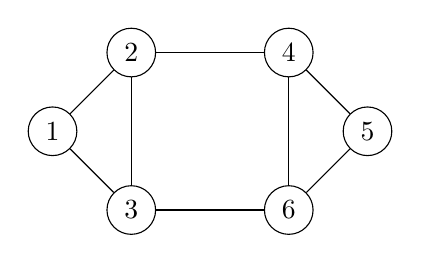
\begin{tikzpicture}[
            % empty/.style={coordinate, draw=white!0, fill=white!0, thin, minimum size = 0.1mm},
            % roundnode/.style={circle, draw=black!60, very thick, minimum size=7mm},
            auto
        ]
            \begin{scope}[
                every node/.style={circle, thin, draw}
            ]
                % Vertices
                \node (p1) at ( 0, 0) {1};
                \node (p2) at ( 1, 1) {2};
                \node (p3) at ( 1,-1) {3};
                \node (p4) at ( 3, 1) {4};
                \node (p5) at ( 4, 0) {5};
                \node (p6) at ( 3,-1) {6};
                % Edges
                \draw[-] (p1) -- (p2); % E1 = (1,2)
                \draw[-] (p1) -- (p3); % E2 = (1,3)
                \draw[-] (p2) -- (p3); % E3 = (2,3)
                \draw[-] (p2) -- (p4); % E4 = (2,4)
                \draw[-] (p4) -- (p5); % E5 = (4,5)
                \draw[-] (p5) -- (p6); % E6 = (5,6)
                \draw[-] (p3) -- (p6); % E7 = (3,6)
                \draw[-] (p4) -- (p6); % E8 = (4,6)
            \end{scope}
        \end{tikzpicture}
    }
    \caption{Graph $G_1$}
\end{figure}

\[
    E = \qty{
        (1,2),
        (1,3),
        (2,3),
        (2,4),
        (4,5),
        (5,6),
        (3,6),
        (4,6)
    }
\]\[
    P_0 = \qty{
        ( 0, 0),
        ( 1, 1),
        ( 1,-1),
        ( 3, 1),
        ( 4, 0),
        ( 3,-1)
    }
\]\[
    R(P_0) = \mqty[
        (x_1 - x_2) & -(x_1 - x_2) & 0              & 0              & 0              & 0              \\
        (x_1 - x_3) & 0              & -(x_1 - x_3) & 0              & 0              & 0              \\
        0             & (x_2 - x_3)  & -(x_2 - x_3) & 0              & 0              & 0              \\
        0             & (x_2 - x_4)  & 0              & -(x_2 - x_4) & 0              & 0              \\
        0             & 0              & 0              & (x_4 - x_5)  & -(x_4 - x_5) & 0              \\
        0             & 0              & (x_3 - x_6)  & 0              & 0              & -(x_3 - x_6) \\
        0             & 0              & 0              & (x_4 - x_6)  & 0              & -(x_4 - x_6)
    ]
\]\[
    R(P_0) = -\mqty[
        -1 & 1  &    &    &    &    \\
        -1 & 1  &    &    &    &    \\
        -1 &    & 1  &    &    &    \\
        1  &    & -1 &    &    &    \\
        & 0  & 0  &    &    &    \\
        & 2  & -2 &    &    &    \\
        & -2 &    & 2  &    &    \\
        & 0  &    & 0  &    &    \\
        &    &    & 1  & -1 &    \\
        &    &    & -1 & 1  &    \\
        &    &    &    & -1 & 1  \\
        &    &    &    & -1 & 1  \\
        &    & 2  &    &    & -2 \\
        &    & 0  &    &    & 0  \\
        &    &    & 0  &    & 0  \\
        &    &    & -2 &    & 2 
    ] \implies \rank(R(P_0) = 8 < 9 = 2 N -3
    \implies G_1 \text{ is not rigid}
\]

\newpage
% G_2 -------------------------------------------------
\subsection{$G_2$}
\begin{figure}[h]
    \label{fig:G_2}
    \centering
    \resizebox*{0.4\textwidth}{!}{
        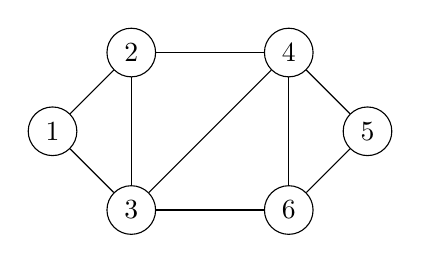
\begin{tikzpicture}[
            % empty/.style={coordinate, draw=white!0, fill=white!0, thin, minimum size = 0.1mm},
            % roundnode/.style={circle, draw=black!60, very thick, minimum size=7mm},
            auto
        ]
            \begin{scope}[
                every node/.style={circle, thin, draw}
            ]
                % Vertices
                \node (p1) at ( 0, 0) {1};
                \node (p2) at ( 1, 1) {2};
                \node (p3) at ( 1,-1) {3};
                \node (p4) at ( 3, 1) {4};
                \node (p5) at ( 4, 0) {5};
                \node (p6) at ( 3,-1) {6};
                % Edges
                \draw[-] (p1) -- (p2); % E1 = (1,2)
                \draw[-] (p1) -- (p3); % E2 = (1,3)
                \draw[-] (p2) -- (p3); % E3 = (2,3)
                \draw[-] (p2) -- (p4); % E4 = (2,4)
                \draw[-] (p4) -- (p5); % E5 = (4,5)
                \draw[-] (p5) -- (p6); % E6 = (5,6)
                \draw[-] (p3) -- (p6); % E7 = (3,6)
                \draw[-] (p4) -- (p6); % E8 = (4,6)
                \draw[-] (p3) -- (p4); % E9 = (3,4)
            \end{scope}
        \end{tikzpicture}
    }
    \caption{Graph $G_2$}
\end{figure}


\[
    E = \qty{
        (1,2),
        (1,3),
        (2,3),
        (2,4),
        (4,5),
        (5,6),
        (3,6),
        (4,6),
        (3,4)
    }
\]\[
    P_0 = \qty{
        ( 0, 0),
        ( 1, 1),
        ( 1,-1),
        ( 3, 1),
        ( 4, 0),
        ( 3,-1)
    }
\]\[
    R(P_0) = \mqty[
        x\_1 - x\_2) & -(x\_1 - x\_2) & 0              & 0              & 0              & 0              \\
        (x\_1 - x\_3) & 0              & -(x\_1 - x\_3) & 0              & 0              & 0              \\
        0             & (x\_2 - x\_3)  & -(x\_2 - x\_3) & 0              & 0              & 0              \\
        0             & (x\_2 - x\_4)  & 0              & -(x\_2 - x\_4) & 0              & 0              \\
        0             & 0              & 0              & (x\_4 - x\_5)  & -(x\_4 - x\_5) & 0              \\
        0             & 0              & (x\_3 - x\_6)  & 0              & 0              & -(x\_3 - x\_6) \\
        0             & 0              & 0              & (x\_4 - x\_6)  & 0              & -(x\_4 - x\_6) \\
        0             & 0              & (x\_3 - x\_4)  & -(x\_3 - x\_4) & 0              & 0   
    ]
\]\[
    R(P_0) = -\mqty[
        -1 & 1  &    &    &    &    \\
        -1 & 1  &    &    &    &    \\
        -1 &    & 1  &    &    &    \\
        1  &    & -1 &    &    &    \\
           & 0  & 0  &    &    &    \\
           & 2  & -2 &    &    &    \\
           & -2 &    & 2  &    &    \\
           & 0  &    & 0  &    &    \\
           &    &    & 1  & -1 &    \\
           &    &    & -1 & 1  &    \\
           &    &    &    & -1 & 1  \\
           &    &    &    & -1 & 1  \\
           &    & 2  &    &    & -2 \\
           &    & 0  &    &    & 0  \\
           &    &    & 0  &    & 0  \\
           &    &    & -2 &    & 2  \\
           &    & 2  & -2 &    &    \\
           &    & 2  & -2 &    &   
    ] \implies \rank(R(P_0) = 9 = 2 N -3
    \implies G_2 \text{ is rigid}
\]


\newpage
% G_3 -------------------------------------------------
\subsection{$G_3$}
\begin{figure}[h]
    \label{fig:G_3}
    \centering
    \resizebox*{0.4\textwidth}{!}{
        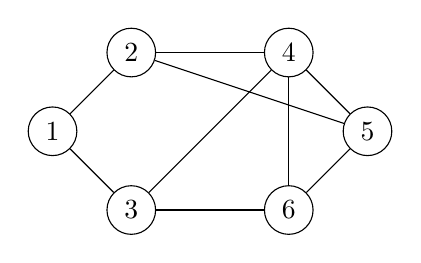
\begin{tikzpicture}[
            % empty/.style={coordinate, draw=white!0, fill=white!0, thin, minimum size = 0.1mm},
            % roundnode/.style={circle, draw=black!60, very thick, minimum size=7mm},
            auto
        ]
            \begin{scope}[
                every node/.style={circle, thin, draw}
            ]
                % Vertices
                \node (p1) at ( 0, 0) {1};
                \node (p2) at ( 1, 1) {2};
                \node (p3) at ( 1,-1) {3};
                \node (p4) at ( 3, 1) {4};
                \node (p5) at ( 4, 0) {5};
                \node (p6) at ( 3,-1) {6};
                % Edges
                \draw[-] (p1) -- (p2); % E1 = (1,2)
                \draw[-] (p1) -- (p3); % E2 = (1,3)
                \draw[-] (p2) -- (p4); % E3 = (2,4)
                \draw[-] (p4) -- (p5); % E4 = (4,5)
                \draw[-] (p5) -- (p6); % E5 = (5,6)
                \draw[-] (p3) -- (p6); % E6 = (3,6)
                \draw[-] (p4) -- (p6); % E7 = (4,6)
                \draw[-] (p3) -- (p4); % E8 = (3,4)
                \draw[-] (p2) -- (p5); % E9 = (2,5)
            \end{scope}
        \end{tikzpicture}
    }
    \caption{Graph $G_3$}
\end{figure}

\[
    E = \qty{
        (1,2),
        (1,3),
        (2,4),
        (4,5),
        (5,6),
        (3,6),
        (4,6),
        (3,4),
        (2,5)
    }
\]\[
    P_0 = \qty{
        ( 0, 0),
        ( 1, 1),
        ( 1,-1),
        ( 3, 1),
        ( 4, 0),
        ( 3,-1)
    }
\]\[
    R(P_0) = \mqty[
        (x\_1 - x\_2) & -(x\_1 - x\_2) & 0              & 0              & 0              & 0              \\
        (x\_1 - x\_3) & 0              & -(x\_1 - x\_3) & 0              & 0              & 0              \\
        0             & (x\_2 - x\_4)  & 0              & -(x\_2 - x\_4) & 0              & 0              \\
        0             & 0              & 0              & (x\_4 - x\_5)  & -(x\_4 - x\_5) & 0              \\
        0             & 0              & (x\_3 - x\_6)  & 0              & 0              & -(x\_3 - x\_6) \\
        0             & 0              & 0              & (x\_4 - x\_6)  & 0              & -(x\_4 - x\_6) \\
        0             & 0              & (x\_3 - x\_4)  & -(x\_3 - x\_4) & 0              & 0              \\
        0             & (x\_2 - x\_5)  & 0              & 0              & -(x\_2 - x\_5) & 0             & 0   
    ]
\]\[
    R(P_0) = -\mqty[
        -1 & 1  &    &    &    &    \\
        -1 & 1  &    &    &    &    \\
        -1 &    & 1  &    &    &    \\
        1  &    & -1 &    &    &    \\
        & -2 &    & 2  &    &    \\
        & 0  &    & 0  &    &    \\
        &    &    & 1  & -1 &    \\
        &    &    & -1 & 1  &    \\
        &    &    &    & -1 & 1  \\
        &    &    &    & -1 & 1  \\
        &    & 2  &    &    & -2 \\
        &    & 0  &    &    & 0  \\
        &    &    & 0  &    & 0  \\
        &    &    & -2 &    & 2  \\
        &    & 2  & -2 &    &    \\
        &    & 2  & -2 &    &    \\
        & 3  &    &    & -3 &    \\
        & -1 &    &    & 1  & 
    ] \implies \rank(R(P_0) = 9 = 2 N -3
    \implies G_3 \text{ is rigid}
\]



% Problem 3 ---------------------------------------
\newpage
\section{}
We can ``grow''  a minimally rigid graph by adding nodes one by one using \emph{\underline{Henneberg construction}}.
\subsection*{Preliminaries}
\begin{definition}
    $G_f$ is considered \emph{\underline{minimally rigid}} if it is rigid and the removal of any single edge renders it not rigid.
\end{definition}

\begin{theorem}
    $G_f$ is minimally rigid if and only if it is rigid and contains \[
        \begin{cases}
            2N - 3 \ \text{edges} & d=2\\
            3N - 6 \ \text{edges} & d=3
        \end{cases}
    \]
\end{theorem}

\subsection{}
\subsubsection*{Problem:}
Briefly state the two rules of Henneberg construction (vertex addition and vertex split) by consulting pages 16 and 17 of Notes 12\_3 uploaded at the elearning page. 
You  can  also  consult  page  6  of  the  reference  [1]  (which  is  also  uploaded  at  the elearning course page). 
[1] B. Anderson, et al. "Rigid graph control architectures for autonomous formations." IEEE Control Systems Magazine 28.6 (2008): 48-63.

\subsubsection*{Solution:}
Given a seed graph that is already minimally rigid, you ``grow'' the graph in two steps:
\begin{enumerate}
    \item \textbf{Vertex Addition:}
    \begin{itemize}
        \item Starts as $(i,j) \in E$        
        \item Add new vertex $v$
        \item Connect $v$ to two adjacent vertices $i$ and $j$
        \item Ends with $(i,j), (v,i), (v,j) \in E$
    \end{itemize}
    \item \textbf{Edge Splitting:}
    \begin{itemize}
        \item Starts as $(i,j), (j,k) \in E$        
        \item Add new vertex $v$
        \item Connect $v$ to vertices $i$, $j$, and $k$ (i.e.) add $(v,i), (v,j), (v,k)$
        \item Remove one of the edges that previously existed (i.e.) remove either $(i,j)$ or $(j,k)$.
        \item Ends with $(i,j), (v,i), (v,j) (v,k) \in E$ or $(j,k), (v,i), (v,j) (v,k) \in E$
    \end{itemize}
\end{enumerate}

\newpage
\subsection{}
\subsubsection*{Problem:}
Starting with the seed graph on the left, obtain the minimally rigid graph on the right by  applying the Henneberg construction rules. 
Clearly state the rule used in each step. 
\begin{figure}[h]
    \centering
    \includegraphics[width = 0.5 \textwidth]{figs/pblm3b_pblm.png}
\end{figure}

\subsubsection*{Solution:}

\textbf{Note:} Due to a lack of time this week, hand drawings were used. 
If too difficult to view or explanation is lacking then I can share the TikZ version in the future.

\begin{figure}[h]
    \centering
    \includegraphics[width=0.25\textwidth]{figs/pblm3b_1.png}
    \includegraphics[width=0.25\textwidth]{figs/pblm3b_2.png}
    \caption{Hand Drawings of Henneberg Construction method for Problem 3b}
\end{figure}

\newpage
\subsection{}
\subsubsection*{Problem:}
Repeat the same problem (as in part (B)) for the following:
\begin{figure}[h]
    \centering
    \includegraphics[width = 0.5 \textwidth]{figs/pblm3c_pblm.png}
\end{figure}

\subsubsection*{Solution:}

\begin{figure}[h]
    \centering
    \includegraphics[width=0.25\textwidth]{figs/pblm3c_1.png}
    \includegraphics[width=0.25\textwidth]{figs/pblm3c_2.png}
    \caption{Hand Drawings of Henneberg Construction method for Problem 3c}
\end{figure}


% Problem 4 ---------------------------------------
\newpage
\section{}
\subsection*{Preliminaries}

\begin{definition} \label{def:tree_graph}
    A graph $G = (V, E)$ is considered a \emph{\underline{Tree}} if it satisfies any of the following equivalent conditions.
    \begin{itemize}
        \item $G$ is connected and acyclic (contains no cycles).
        \item $G$ is acyclic, and a cycle is formed if any edge is added.
        \item $G$ is connected, but would be disconnected if any edge is removed.
        % \item $G$ is connected and $K_3$ is not a minor of $T$.
        \item Any two vertices in $G$ can be connected by a unique simple path.
    \end{itemize}
    If $G$ is a finite graph with $N$ vertices, then these additional conditions are also equivalent:
    \begin{itemize}
        \item $G$ is connected and has $N - 1$ edges.
        % \item G is connected, and every subgraph of G includes at least one vertex with zero or one incident edges. (That is, G is connected and 1-degenerate.)
        \item $G$ has no simple cycles and has $N-1$ edges.
    \end{itemize}
\end{definition}

\subsection*{Problem}
Let's consider two trees $T_1 = (V, E_1)$ and $T_2 = (V, E_2)$ that have the same vertex sets containing $N$ vertices, but possibly different edge sets. 
Is it possible that the union of two such trees result in a minimally rigid graph? 
If yes, explain and construct an example. 
If not, explain why not. 

\subsection*{Solution}
By definition, a tree will have exactly $N-1$ edges. 
One necessary condition for a minimally rigid graph, when $d=2$, is to have $2N-3$ edges, which is possible as $T_1 \cup T_2$ would contain $\leq 2N - 2$ edges.
Additionally, within all connected graphs there exists induced subgraphs that are trees, so in many\footnote{
    mabye all, but I don't have a proof for that
} minimally rigid graphs there will be two distinct trees that can be defined to be $T_1$ and $T_2$.

Regardless, the answer is \textbf{YES}. 
See \figurename{\ref{fig:pblm4_1}}, \figurename{\ref{fig:pblm4_2}}, and \figurename{\ref{fig:pblm4_3}} for an example.

\newpage
\begin{figure}[h]
    \centering
    \resizebox*{0.4\textwidth}{!}{
        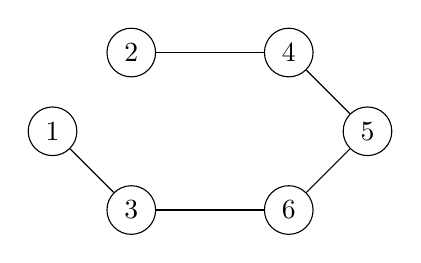
\begin{tikzpicture}[
            % empty/.style={coordinate, draw=white!0, fill=white!0, thin, minimum size = 0.1mm},
            % roundnode/.style={circle, draw=black!60, very thick, minimum size=7mm},
            auto
        ]
            \begin{scope}[
                every node/.style={circle, thin, draw}
            ]
                % Vertices
                \node (p1) at ( 0, 0) {1};
                \node (p2) at ( 1, 1) {2};
                \node (p3) at ( 1,-1) {3};
                \node (p4) at ( 3, 1) {4};
                \node (p5) at ( 4, 0) {5};
                \node (p6) at ( 3,-1) {6};
                % Edges
                % \draw[-] (p1) -- (p2); % E1 = (1,2)
                \draw[-] (p1) -- (p3); % E2 = (1,3)
                % \draw[-] (p2) -- (p3); % E3 = (2,3)
                \draw[-] (p2) -- (p4); % E4 = (2,4)
                \draw[-] (p4) -- (p5); % E5 = (4,5)
                \draw[-] (p5) -- (p6); % E6 = (5,6)
                \draw[-] (p3) -- (p6); % E7 = (3,6)
                % \draw[-] (p4) -- (p6); % E8 = (4,6)
                % \draw[-] (p3) -- (p4); % E9 = (3,4)
            \end{scope}
        \end{tikzpicture}
    }
    \caption{Graph $T_1$}
    \label{fig:pblm4_1}
\end{figure}
    
\begin{figure}[h]
    \centering
    \resizebox*{0.4\textwidth}{!}{
        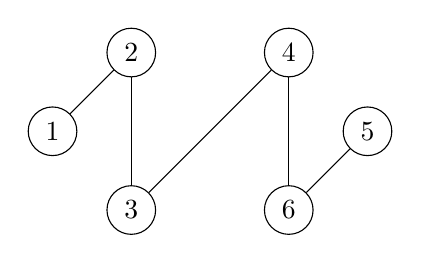
\begin{tikzpicture}[
            % empty/.style={coordinate, draw=white!0, fill=white!0, thin, minimum size = 0.1mm},
            % roundnode/.style={circle, draw=black!60, very thick, minimum size=7mm},
            auto
        ]
            \begin{scope}[
                every node/.style={circle, thin, draw}
            ]
                % Vertices
                \node (p1) at ( 0, 0) {1};
                \node (p2) at ( 1, 1) {2};
                \node (p3) at ( 1,-1) {3};
                \node (p4) at ( 3, 1) {4};
                \node (p5) at ( 4, 0) {5};
                \node (p6) at ( 3,-1) {6};
                % Edges
                \draw[-] (p1) -- (p2); % E1 = (1,2)
                % \draw[-] (p1) -- (p3); % E2 = (1,3)
                \draw[-] (p2) -- (p3); % E3 = (2,3)
                % \draw[-] (p2) -- (p4); % E4 = (2,4)
                % \draw[-] (p4) -- (p5); % E5 = (4,5)
                \draw[-] (p5) -- (p6); % E6 = (5,6)
                % \draw[-] (p3) -- (p6); % E7 = (3,6)
                \draw[-] (p4) -- (p6); % E8 = (4,6)
                \draw[-] (p3) -- (p4); % E9 = (3,4)
            \end{scope}
        \end{tikzpicture}
    }
    \caption{Graph $T_2$}
    \label{fig:pblm4_2}
\end{figure}
    
\begin{figure}[h]
    \centering
    \resizebox*{0.4\textwidth}{!}{
        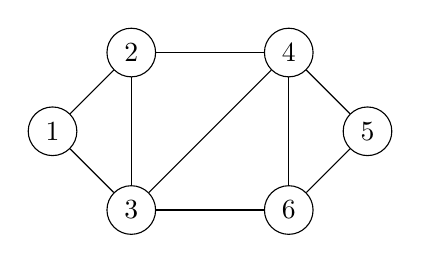
\begin{tikzpicture}[
            % empty/.style={coordinate, draw=white!0, fill=white!0, thin, minimum size = 0.1mm},
            % roundnode/.style={circle, draw=black!60, very thick, minimum size=7mm},
            auto
        ]
            \begin{scope}[
                every node/.style={circle, thin, draw}
            ]
                % Vertices
                \node (p1) at ( 0, 0) {1};
                \node (p2) at ( 1, 1) {2};
                \node (p3) at ( 1,-1) {3};
                \node (p4) at ( 3, 1) {4};
                \node (p5) at ( 4, 0) {5};
                \node (p6) at ( 3,-1) {6};
                % Edges
                \draw[-] (p1) -- (p2); % E1 = (1,2)
                \draw[-] (p1) -- (p3); % E2 = (1,3)
                \draw[-] (p2) -- (p3); % E3 = (2,3)
                \draw[-] (p2) -- (p4); % E4 = (2,4)
                \draw[-] (p4) -- (p5); % E5 = (4,5)
                \draw[-] (p5) -- (p6); % E6 = (5,6)
                \draw[-] (p3) -- (p6); % E7 = (3,6)
                \draw[-] (p4) -- (p6); % E8 = (4,6)
                \draw[-] (p3) -- (p4); % E9 = (3,4)
            \end{scope}
        \end{tikzpicture}
    }
    \caption{Graph $T_1 \cup T_2$}
    \label{fig:pblm4_3}
\end{figure}


% Problem 5 ---------------------------------------
\newpage
\section{}
In class, we saw that if we place a total of $(P + 2)$ agents on a line, with $P$ agents at location 0, one agent at location $\Delta$, and one agent at location $2\Delta$, then if the network is a $\Delta$-disk proximity graph it will get disconnected under the linear consensus equation if $P > 2$.

% Part a
\subsection{}
\subsubsection*{Problem}
Show that this particular configuration is indeed the worst-case scenario from a connectivity point-of-view.

\subsubsection*{Solution}
As far as the definition of the $\Delta$-disk proximity graph goes, the positioning of $v_1$ at $2 \Delta$ and $v_2$ at $\Delta$ places them at the exact point of disconnection. 
Additionally, having the points $v_{i = 3, \dots, 2+P}$ at $0$ places them at the extreme to maximize the consensus `pull' on $v_2$.
This results in the worst-case scenario where $v_2$ is `pulled' as hard as allowed by the $\Delta$-disk proximity graph definition, while the $v_1$ and $v_2$ edge is already at it's `breaking point'.

% Part b
\subsection{}
\subsubsection*{Problem}
Is the following theorem valid? 
A $\Delta$-disk proximity graph network of 4 agents will always stay connected under the consensus equation if it starts connected.

\subsubsection*{Solution}
Technically yes. 
Since in this case $P=2$, $\dot{x}_2 = (1 - 2) \Delta = - \Delta$ (which is equal to $\dot{x}_1 = - \Delta$) and therefore they will maintain a distance smaller than $\Delta$ and remain connected.





% Problem 6------------------
\newpage
\section{}
See attached MATLAB File for code.

\subsection{Problem}
\subsubsection{}
Make sure that the network stays connected for all three initial networks. 
(I am not looking for a proof here - just try and be clever and produce some appropriate control law that works in simulation.)


\textbf{Proposed Solution:}
No need to be clever since the edge-tension algorithm is already implemented which guarantees that once a connection exists it will not disappear.
The Hysteresis that is implemented does make it so that it isn't great near the outskirts but it works regardless.

An option (as tested) to improve the far away ones without making Hysteresis infinite, is to add a standard baseline weight if an edge exists but is still out of range. (i.e)
\begin{figure}[h]
    \centering
    \includegraphics[]{figs/pblm6a_code.png}
\end{figure}

\subsubsection{}
Make  sure  that  the  agents  do  not  run  into  each  other,  i.e.,  that  collisions  are avoided, at the same time as the network remains connected. 
Again, I do not want a proof I want the simulations to work

\textbf{Proposed Solution:}
The edge-tension algorithm also already takes care of this for the most part. 
An additional modification of the Hysteresis function component can allow for more of a 'motivator' to force the agents to stay away from each other.
\begin{figure}[h]
    \centering
    \includegraphics[width=0.4 \textwidth]{figs/pblm6b_code.png}
\end{figure}

\newpage
\subsection{Network 1 Results}
\begin{figure}[h]
    \centering
    \includegraphics[height = 0.75 \textheight]{figs/pblm6_network1.png}
\end{figure}


\newpage
\subsection{Network 2 Results}
\begin{figure}[h]
    \centering
    \includegraphics[height = 0.75 \textheight]{figs/pblm6_network2.png}
\end{figure}


\newpage
\subsection{Network 3 Results}
\begin{figure}[h]
    \centering
    \includegraphics[height = 0.75 \textheight]{figs/pblm6_network3.png}
\end{figure}


\newpage
\appendix
\section{MATLAB Code:}\label{apx:matlab}
All code I write in this course can be found on my GitHub repository:\\
\href{https://github.com/jonaswagner2826/MECH6V29_MultiagentRoboticSystems}{https://github.com/jonaswagner2826/MECH6V29\_MultiagentRoboticSystems}

% \bibliographystyle{ieeetran}
% % \bibliography{refs.bib}
% \cite{*}

% \includepdf[pages=-]{MECH6V29_HW03.pdf}
% \includepdf[pages=-, nup = 2x2]{MECH6V29_HW03.pdf}


\end{document}
